%%%%%%
%
% $Autor: ter Veen $
% $Datum: 01.06.2024 $
% $Version: 1 $
% $Pfad: SchrittmotorArduino/DevoloperDoc/tikz/ArduinoPinout.tex $
%
%%%%%%
	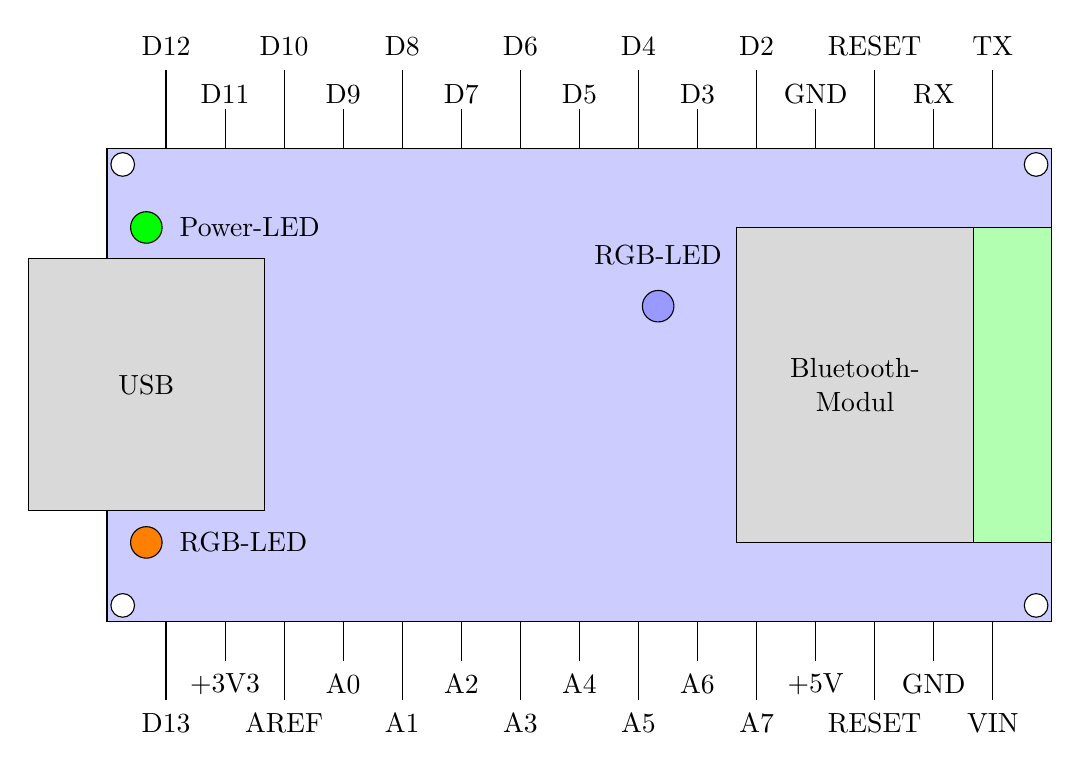
\begin{tikzpicture}[scale=2]
		% Arduino Dummy
		\draw[fill=blue!20] (0,0) rectangle (6,3);
		
		% Pin Beschriftung oben
		\foreach \x in {0.375,1.125,...,5.625}
		\draw (\x,3) -- (\x,3.5) node[above] {};
		\foreach \x in {0.75,1.5,...,5.25}
		\draw (\x,3) -- (\x,3.25) node[above] {};
		
		% Pin Beschriftung unten
		\foreach \x in {0.375,1.125,...,5.625}
		\draw (\x,0) -- (\x,-0.5) node[below] {};
		\foreach \x in {0.75,1.5,...,5.25}
		\draw (\x,0) -- (\x,-0.25) node[below] {};
		
		
		% Pins oben
		\node at (0.375,3.65) {D12};
		\node at (0.75,3.35) {D11};
		\node at (1.125,3.65) {D10};
		\node at (1.5,3.35) {D9};
		\node at (1.875,3.65) {D8};
		\node at (2.25,3.35) {D7};
		\node at (2.625,3.65) {D6};
		\node at (3,3.35) {D5};
		\node at (3.375,3.65) {D4};
		\node at (3.75,3.35) {D3};
		\node at (4.125,3.65) {D2};
		\node at (4.5,3.35) {GND};
		\node at (4.875,3.65) {RESET};
		\node at (5.25,3.35) {RX};
		\node at (5.625,3.65) {TX};
		
		% Pins unten
		\node at (0.375,-0.65) {D13};
		\node at (0.75,-0.4) {+3V3};
		\node at (1.125,-0.65) {AREF};
		\node at (1.5,-0.4) {A0};
		\node at (1.875,-0.65) {A1};
		\node at (2.25,-0.4) {A2};
		\node at (2.625,-0.65) {A3};
		\node at (3,-0.4) {A4};
		\node at (3.375,-0.65) {A5};
		\node at (3.75,-0.4) {A6};
		\node at (4.125,-0.65) {A7};
		\node at (4.5,-0.4) {+5V};
		\node at (4.875,-0.65) {RESET};
		\node at (5.25,-0.4) {GND};
		\node at (5.625,-0.65) {VIN};
		
		% Dummys zur Orientierung
	
		\draw[fill=gray!30] (4,0.5) rectangle (5.5,2.5) node[pos=0.5, align=center] {Bluetooth-\\Modul};
		\draw[fill=green!30] (5.5,0.5) rectangle (6,2.5) node[pos=0.5, align=center] {};
		\draw[fill=gray!30] (-0.5,0.7) rectangle (1,2.3) node[pos=0.5, align=center] {USB};
		\draw[fill=white] (0.1,2.9) circle (0.075) node[right=1mm]{};
		\draw[fill=white] (0.1,0.1) circle (0.075) node[right=1mm]{};
		\draw[fill=white] (5.9,0.1) circle (0.075) node[right=1mm]{};
		\draw[fill=white] (5.9,2.9) circle (0.075) node[right=1mm]{};
		
		% LED´s
		\draw[fill=green] (0.25,2.5) circle (0.1) node[right=3mm] {Power-LED};
		\draw[fill=orange] (0.25,0.5) circle (0.1) node[right=3mm] {RGB-LED};
		\draw[fill=blue!40] (3.5,2) circle (0.1) node[above=4mm] {RGB-LED};
		
	\end{tikzpicture}
